\documentclass{article}
\usepackage[utf8]{inputenc} %кодировка
\usepackage[T2A]{fontenc}
\usepackage[english,russian]{babel} %русификатор 
\usepackage{mathtools} %библиотека матеши
\usepackage[left=1cm,right=1cm,top=2cm,bottom=2cm,bindingoffset=0cm]{geometry} %изменение отступов на листе
\usepackage{amsmath}
\usepackage{graphicx} %библиотека для графики и картинок
\graphicspath{}
\DeclareGraphicsExtensions{.pdf,.png,.jpg}
\usepackage{subcaption}
\usepackage{pgfplots}
\usepackage{amssymb}
\usepackage{physics}

\begin{document}


\section{ФНП и скалярное поле
П.1 Основные понятия}


$\mathbb{R} x \mathbb{R} x \mathbb{R} ... x \mathbb{R} = \mathbb{R}^n = \{(x_1, x_2, .., x_n): x_i \in \mathbb{R}, i = 1 ... n\}\\
\mathbb{D} \in \mathbb{R}^n \\
n = 2 (x,y)$


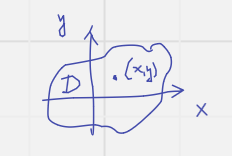
\includegraphics[width=.3\textwidth]{1.1} 



Ограниченность $\mathbb{D} $ - ограничена, если существует  M>0 Для любых $(x, y) \in \mathbb{D} \sqrt{x^2+y^2}\in \leq \delta(M, O) \leq M$

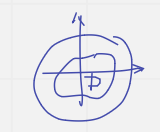
\includegraphics[width=.3\textwidth]{1.2} 

Внутренняя точка (IntD) M(x, y) - внутренняя, если существует $\mathcal{E} > 0 : U_{\mathcal{E}}(M) \in D $ == $\{(x', y'): \sqrt{(x-x')^2+(y-y')} < \mathcal{E}\}$

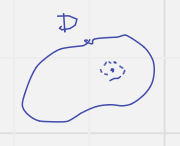
\includegraphics[width=.3\textwidth]{1.3} 

Граничная точка (знак частных производных)$\mathcal{D}$): M(x, y)
- граничная точка, если существует $\mathcal{E} > 0 : U^{\cdot}_{\mathcal{E}}(M) \cap \mathcal{D} != \bar{0}\  and\  U^{\cdot}_{\mathcal{E}}(M) \cap \bar{\mathcal{D}} != \bar{0}$


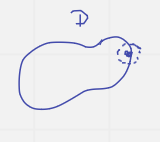
\includegraphics[width=.3\textwidth]{gran} 


Изолированная точка: существует $\mathcal{E} > 0 : U^{\cdot}_{\mathcal{E}}(M) \cap \mathcal{D} = \bar{0}$

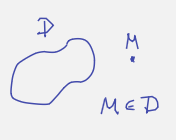
\includegraphics[width=.3\textwidth]{isolate} 


$\mathcal{F}: \mathcal{D} -> \mathbb{R}\ \forall(x, y) \in \mathcal{D}\ and \ \forall(x, y)\in \mathcal{D}\ =>\ !z \in \mathbb{R}: z = f(x,y)$

$\mathcal{D}$ - облать определения

E -множество точек

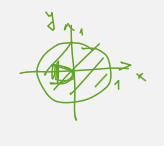
\includegraphics[width=.3\textwidth]{ddd} 
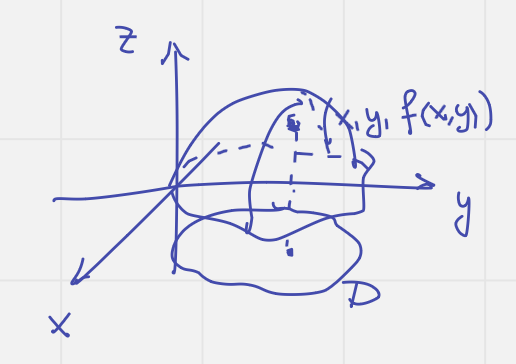
\includegraphics[width=.3\textwidth]{2} 


Г $= \{(x, y, f(x,y)): (x, y) \in \mathcal{D}\}$ -график 

Пример: 
$z = \sqrt{1-x^2-y^2}$

$\mathcal{D} = \{(x, y): x^2 + y ^2 \leq 1\}$


\begin{equation*}
    \begin{cases}
        x^2+y^2+z^2 = 1\\
        z \geq 0
    \end{cases}
\end{equation*}

E = [0; 1]

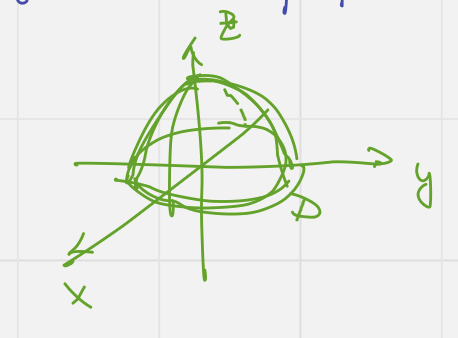
\includegraphics[width=.3\textwidth]{3} 
\\ \\
\section{П.2 Линии и поверхности уровня}

n = 2 $f: \mathcal{D} -> \mathbb{R}$

$L_c = \{(x, y): f(x, y = c )\}$

$S_c = \{(x, y, z): f(x, y, z = c )\}$

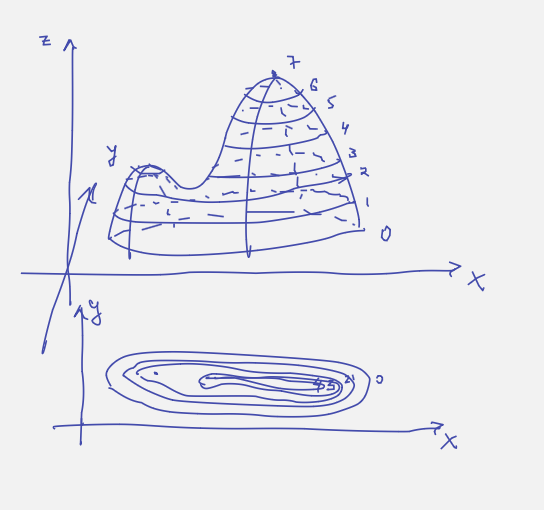
\includegraphics[width=.3\textwidth]{line} 
\\ \\
\section{п.3 Частное и полное приращение }

$f: \mathcal{D} -> \mathbb{R}$, n=2

z = f(x, y)

$\Delta z = f(x+ \Delta x, y + \Delta y) - f(x, y)$

полное приращение

$\Delta_x z = f(x+ \Delta x, y) - f(x, y)$

частное приращение по переменной x

$\Delta_y z = f(x, y + \Delta y) - f(x, y)$

частное приращение по переменной y

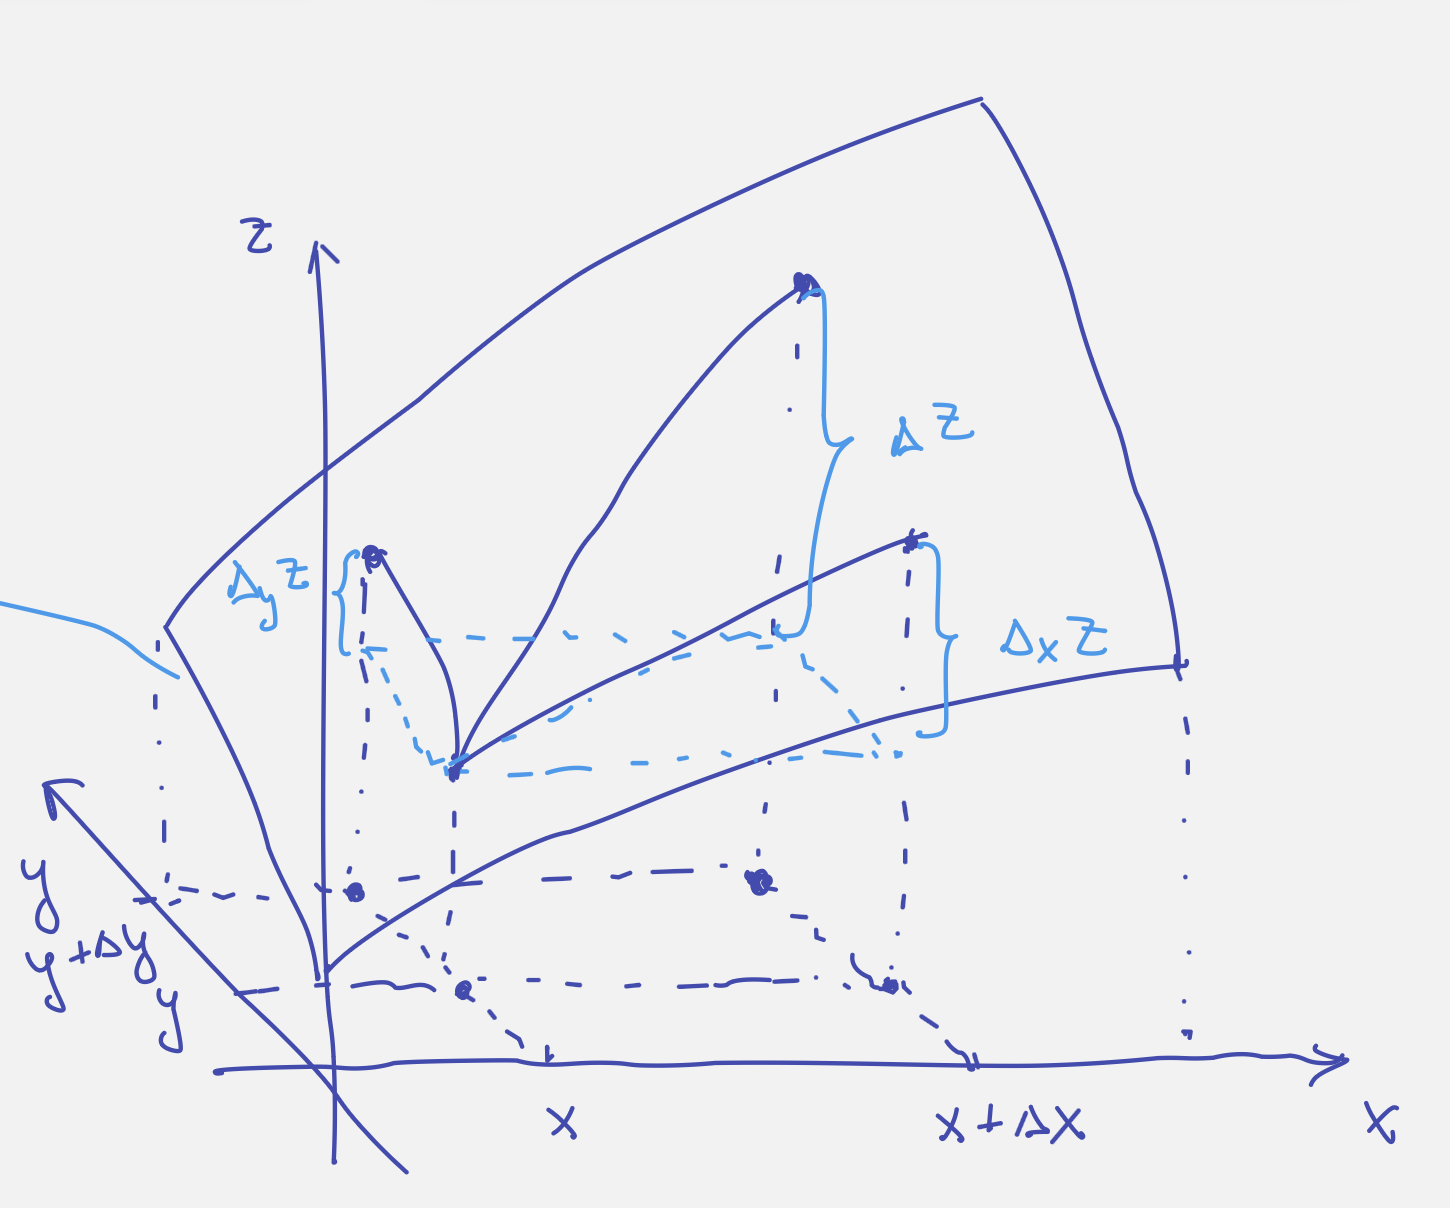
\includegraphics[width=.4\textwidth]{prir.png} 

$\Delta z != \Delta_x z + \Delta_y z $

Пример: 

S = xy

x=1 $\Delta x =0,1 $

y=2 $\Delta y =0,2 $

$\Delta S = (x+\Delta x)(y+\Delta y) - xy = x \Delta y + y \Delta x +\Delta x \Delta y = 0,42$


$\Delta_x S + \Delta_y S = (x + \Delta x)y - xy + (y +\Delta y)x  - xy = \Delta x \cdot y + \Delta y \cdot x$


\section{п.4 Предел и непрерывность }

$\lim_{x -> x_0}f(x) = A\ <=>\ \forall \mathcal{E} >0 \ \exists \delta_{\mathcal{E}}>0 : \forall x \in U^{\cdot}_{\delta}(x_0) \cap \mathcal{D}_f => f(x) \in U_{\mathcal{E}}(A)$


$\lim_{M -> M_0}f(M) = A\ <=>\ \forall \mathcal{E} >0 \ \exists \delta_{\mathcal{E}}>0 : \forall M \in U^{\cdot}_{\delta}(M_0) \cap \mathcal{D}_f => f(M) \in U_{\mathcal{E}}(A)$
\\ \\
$M(x, y), M(x_1, y_1)$
\\ \\
1) $z = x^2 +y^2 \mathcal{D} = \mathbb{R}^2 \Delta z= (x_0 + \Delta x)^2 + (y+ \Delta y)^2 - x_0^2 - y_0^2 = 2x_0 \Delta x + \Delta x^2 +2y_0\Delta y + \Delta y^2 - (\Delta x ->0,  \Delta y ->0) -> 0 $

z - непрерывная на $\mathcal{D} = \mathbb{R}^2$

$\lim_{(x, y)-> 0)}(\frac{2xy}{x^2 +y^2}) = |y = kx| = \lim_{(x, y)-> 0)}(\frac{2xkx}{x^2 +(kx)^2}) = \frac{2k}{1+k^2} предел не существует
$

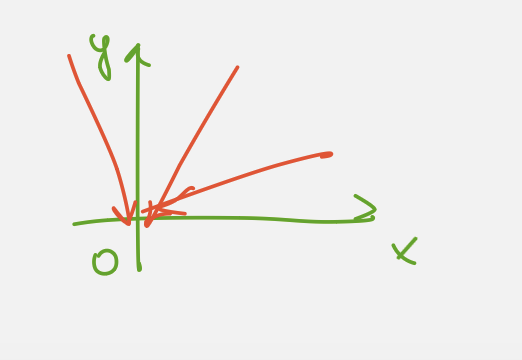
\includegraphics[width=.3\textwidth]{lines} 
\\ \\
\section{П.5 Частные производные}

Обычные случаи 
\begin{equation*}
    z = f(x)\ \dv{z}{x}= \lim_{\Delta x-> 0}\frac{\Delta x}{\Delta y}
\end{equation*}
\begin{center}
    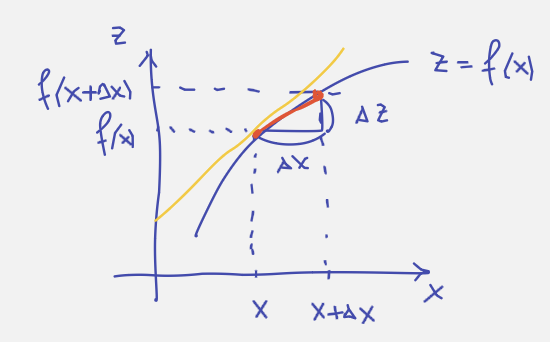
\includegraphics[width=.3\textwidth]{f(x).png} 
\end{center}


Случай с частной производной 
\begin{equation*}
    z = f(x, y)\ \Delta_x z = f(x + \Delta x, y) - f(x, y); \ \ \pdv{z}{x} = \lim_{\Delta x-> 0}\frac{\Delta_x z}{\Delta x}
\end{equation*}
Частная производная функции z по y в точке M(x, y)

\begin{equation*}
    \Delta x - fiks\ => \ \Delta_x z = f(x +\Delta x, y) - f(x, y);\ \pdv{z}{x} = \lim_{\Delta x -> 0 }   \frac{\Delta_x z}{\Delta x}
\end{equation*}
Частная производная функции y по y в точке M(x, y)

\begin{equation*}
    \Delta y - fiks\ => \ \Delta_y z = f(x, y +\Delta y) - f(x, y);\ \pdv{z}{y} = \lim_{\Delta y -> 0 }   \frac{\Delta_y z}{\Delta y}
\end{equation*}
\begin{equation*}
    \pdv{z}{l} = \lim_{\Delta l -> 0 }   \frac{\Delta_l z}{\Delta l}
\end{equation*}
Частная производная функции y по направлению в точке M(x, y)
\begin{center}
    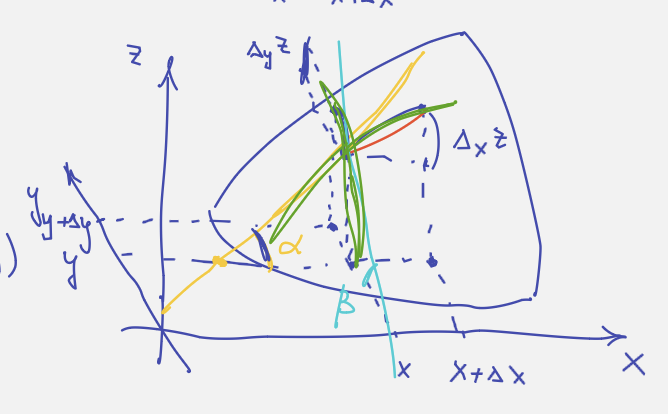
\includegraphics[width=.3\textwidth]{f(x,y).png} 
\end{center}

\section{П.6 Дифферинциал}


\begin{equation*}
    z = f(x);\ \Delta z =A \cdot \Delta x + \alpha(x)\cdot \Delta x = f'(x) + \Delta x = \dd z +o(\Delta x)
\end{equation*}
\begin{center}
    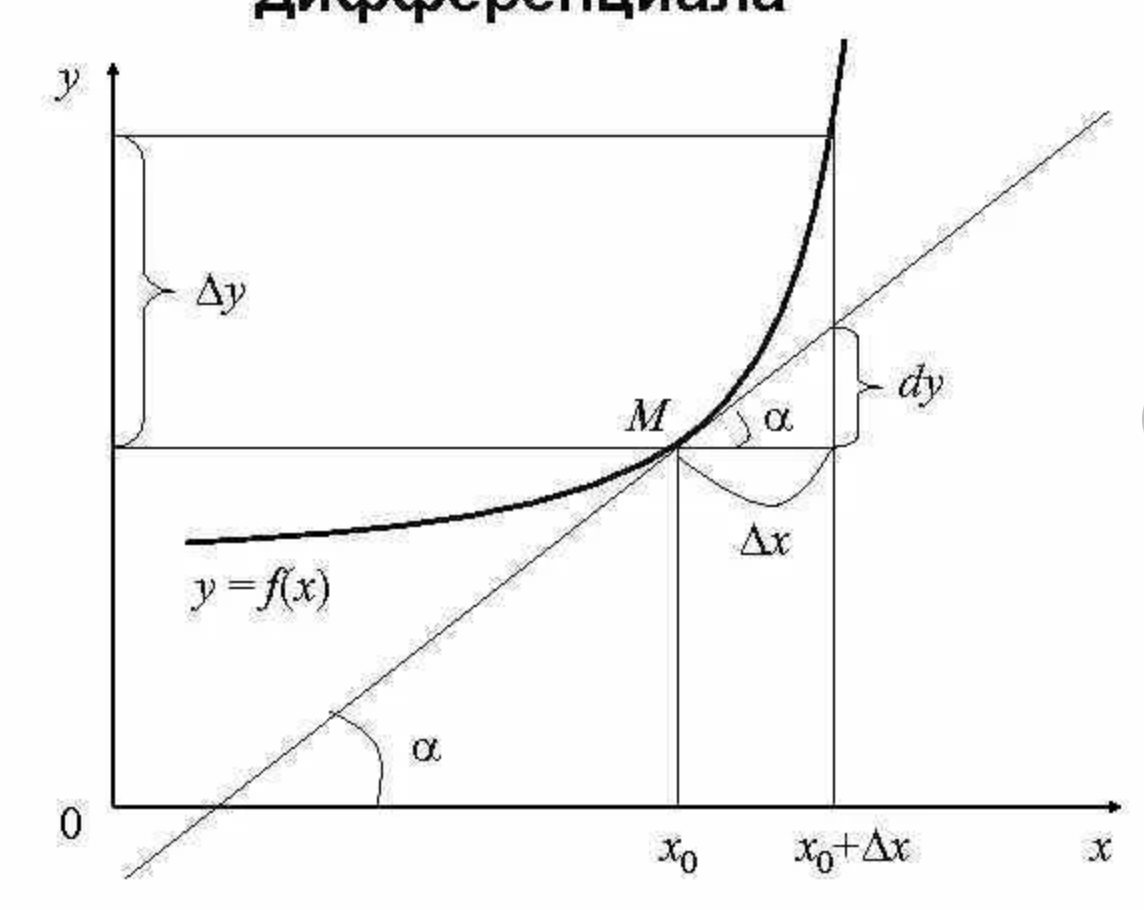
\includegraphics[width=.3\textwidth]{dx} 
\end{center}

Полный Дифферинциал функции двух переменных

\begin{equation*}
    z = f(x, y);\ \Delta z =A \cdot \Delta x + b \cdot \Delta y;\ A, B \in \mathbb{R}
\end{equation*}
\textbf{Теорема(о дифферинциале)}:\\
\begin{equation*}
    z = f(x,y) \ M(x,y)
\end{equation*}
\begin{equation*}
    => \dd z = z_x'\dd x + z_y'\dd y 
\end{equation*}
\begin{equation*}
    \Delta z = \dd z + o(\Delta \rho)
\end{equation*}
Доказательство:\\
\begin{equation*}
    \Delta z = f(x+\Delta x, y +\Delta y) - f(x, y) = (f(x+\Delta x, y + \Delta y) - f(x, y+\Delta y)) + f(x, y+\Delta y)- f(x, y)
\end{equation*}
\begin{equation*}
    \Delta z_1 = f(x, y+\Delta y) - f(x, y) = | x - fiks;\ f(x, y)= \psi(y) | = \psi(y +\Delta y)- \psi (y) = 
\end{equation*}
\begin{equation*}
    =|\psi(y) - \text{непрерывная}; \text{по т. Лагранжа}: \exists \overline{y}: \psi(y + \Delta y) - \psi(y) = \psi'_y(\overline{y}\Delta y) | = 
\end{equation*}
\begin{equation*}
    = \psi'_y(\overline{y}\Delta y) = f'_y(x, \overline{y})\Delta y
\end{equation*}

\begin{equation*}
    \Delta z_2 = f(x + \Delta x, y+  \Delta y) = f(x, y+ \Delta y) = |y+\Delta y - fiks;\ f(x, \Delta y +y) = \phi (x)| = \phi(x + \Delta x) = 
\end{equation*}

\begin{equation*}
    = f'_x(\overline{x}, y+\Delta y)\cdot \Delta x 
\end{equation*}

\begin{equation*}
    => \Delta z = \Delta z_2 +\Delta z_1 = f'_x(\overline{x}, y+\Delta y)\Delta x+ f'_y(x, \overline{y})\Delta y
\end{equation*}

\begin{equation*}
    \measuredangle  \lim_{\Delta x -> 0, \Delta y -> 0}f'_x(\overline{x}, y+\Delta y) = f'_x(x, y)
\end{equation*}
по т. о функции, её предел и бмф:
\begin{equation*}
    f'_x(\overline{x}, y+\Delta y) = f'_x(x, y)+\alpha(\Delta \rho)
\end{equation*}
\begin{equation*}
    \measuredangle  \lim_{\Delta y -> 0}f'_y(x,\overline{y}) = f'_y(x, y)\ => \ f_y'(x, \overline{y}) = f_y'(x, y)+ \beta(\Delta \rho)
\end{equation*}
\begin{equation*}
    = f_x'(x, y)\Delta x+ f_y'(x,y)\Delta y +\alpha (\Delta \rho)\Delta x +\beta(\Delta \rho)\Delta y = \dd z+ o(\Delta \rho)
\end{equation*}
\begin{equation*}
    \dd z = f'_x(x,y)\dd x + f_y'(x,y)\dd y
\end{equation*}
Доказано\\
\section{П.7 Производная сложной функции, полная производная, полный Дифферинциал}
\begin{equation}
    z = z(u,v),\ u = u(x, y),\ v = v(x,y)
\end{equation}
\begin{equation}
    z = z(u, v)= z(u(x,y), v(x,y)) = f(x,y)
\end{equation}
Теорема о производной сложной ф
\begin{equation}
    z(u,v),\ u(x,y)\ v(x,y)
\end{equation}
\begin{equation}
    => \pdv{z}{x} = \pdv{z}{u}\cdot \pdv{u}{x} + \pdv{z}{v}\cdot \pdv{v}{x}
\end{equation}
\begin{equation}
     \pdv{z}{y} = \pdv{z}{u}\cdot \pdv{u}{y} + \pdv{z}{v}\cdot \pdv{v}{y}
\end{equation}
\begin{center}
    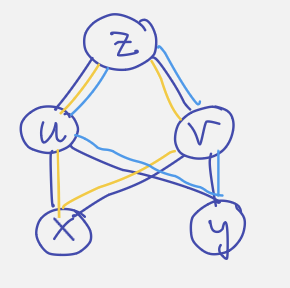
\includegraphics[width=.3\textwidth]{graphF.png} 
\end{center}
докажем
\begin{equation}
    \measuredangle \pdv{z}{x}:
\end{equation}
\begin{equation}
    \Delta x -> \Delta_x u, \Delta_x v-> \Delta z;\ y -fiks
\end{equation}
\begin{equation}
    \Delta z= \pdv{z}{u}\Delta_x u +\pdv{z}{v}\Delta_xv+\alpha(\Delta_xu)\Delta_xu+\beta(\Delta_xv)\Delta_xv\ \ \ |:\Delta x
\end{equation}
\begin{equation}
    \frac{\Delta z}{\Delta x} = \pdv{z}{u}\cdot \frac{\Delta_x u}{\Delta x}+\pdv{z}{v}\cdot\frac{\Delta_xv}{\Delta x}+ \alpha(\Delta_x u)\frac{\Delta_xu}{\Delta x} +\beta(\Delta_xv)\frac{\Delta_yv}{\Delta x}
\end{equation}
\begin{equation}
    \lim_{\Delta x->0}: \Delta -> 0 => \text{непрерывна}: \Delta_xu -> 0, \Delta_xv -> 0 => \alpha, \beta -> 0
\end{equation}
\begin{equation}
    \pdv{z}{x} = \pdv{z}{u} \cdot \pdv{u}{x} + \pdv{z}{v}\cdot \pdv{v}{x}
\end{equation}
для $\pdv{z}{y}$ по аналогии\\
\textbf{Доказано}




\section{Производная от функций, заданной неявно}
\begin{equation*}
    y=y(x),\ F(x,y)=0,\ y'
\end{equation*}
Первый способ решения
\begin{equation*}
    e^y-e^x+xy=0\ (e^y-e^x+xy)'_x=0,\ y = y(x)
\end{equation*}
\begin{equation*}
    e^y\cdot y'-e^y+y+xy'=0,\ (e^y+x)y' = e^x-y,\ y' = \frac{e^x-y}{e^y+x}
\end{equation*}
Второй способ решения
\begin{equation}
    y' = -\frac{F'_x(x,y)}{F'_y(x,y)}
\end{equation}
\begin{equation*}
    F'_x(x,y) = -e^x+y
\end{equation*}
\begin{equation*}
    F'_y(x,y) = e^y+x
\end{equation*}
\begin{equation*}
    y' = \frac{-e^x+y}{e^y+x}
\end{equation*}
Теорема о производной функции заданной неявно
\begin{equation*}
    y= y(x)- \text{непрерывна},\ F(x,y) = 0,\ (F,F'_x,F'_y - \text{непрерывны в окр (x,y)})
\end{equation*}
\begin{equation}
    =>\ y' = \frac{F'_x(x,y)}{F'_y(x,y)};\ \dv{y}{x}= -\frac{\pdv{F}{x}(x,y)}{\pdv{F}{y}(x,y)}
\end{equation}
Доказательство
\begin{equation*}
    x;\ y(x);\ F(x,y) = 0
\end{equation*}
-
\begin{equation*}
    \Delta x;\ \Delta y(x);\ F(x+\Delta x,y+\Delta y) = 0
\end{equation*}
=
\begin{equation*}
    \Delta F(x) = F(x+\Delta x; y+ \Delta y) - F(x;y) = 0
\end{equation*}
\begin{equation*}
    \Delta F(x) = \pdv{F}{x}\Delta x + \pdv{F}{y}\Delta y + \alpha(\Delta \rho)\Delta x + \beta (\Delta \rho) \Delta y = 0\ | :\Delta x
\end{equation*}
\begin{equation*}
     \pdv{F}{x} + \pdv{F}{y}\frac{\Delta y}{\Delta x} + \alpha(\Delta \rho) + \beta (\Delta \rho) \frac{\Delta y}{\Delta x} = 0
\end{equation*}
\begin{equation*}
    (\pdv{F}{y} + \beta (\Delta \rho))\frac{\Delta y}{\Delta x} = -(\pdv{F}{x} +\alpha(\Delta \rho))
\end{equation*}
\begin{equation*}
    \frac{\Delta y}{\Delta x} = -\frac{\pdv{F}{x} +\alpha(\Delta \rho)}{\pdv{F}{y} + \beta (\Delta \rho)};\ \Delta x -> 0\ => \Delta y->0,\ \Delta \rho -> 0 \ =>\ \dv{y}{x} = \dv{-\frac{F}{x}}{\pdv{F}{y}}
\end{equation*}
Доказано
\begin{equation*}
    z = z(x,y)\ F(x,y,z)= 0\ z=z(x,y)\ \pdv{z}{x},\ \pdv{z}{y} - ?
\end{equation*}
\begin{equation*}
    \pdv{z}{x} = -\frac{\pdv{F}{x}}{\pdv{F}{z}} \ and\ \pdv{z}{y} = -\frac{\pdv{F}{y}}{\pdv{F}{z}}
\end{equation*}
\begin{equation*}
    z = z(x,y) \text{непрерывная}, F,\ F'_x, \ F'_y, \ F'_z - \ \text{непрерывная}\ and\ F'_z != 0
\end{equation*}
\section{Производная по направлению}
\begin{equation*}
    z = z(x,y),\ M(x;y),\ \overline{l}(l_x;\ l_y)
\end{equation*}
\begin{equation*}
    \Delta x,\ \Delta y\ \text{вдоль }\overline{l}=>M'(x+\Delta x; y+\Delta y);\ \ \frac{\Delta_l z}{\Delta l}\ ->\ \pdv{z}{l}\ (\Delta l -> 0)
\end{equation*}
\begin{center}
    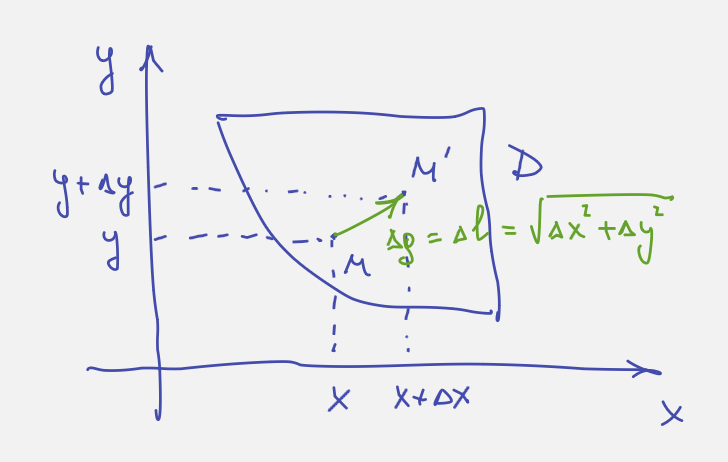
\includegraphics[width=.3\textwidth]{ll.png} 
    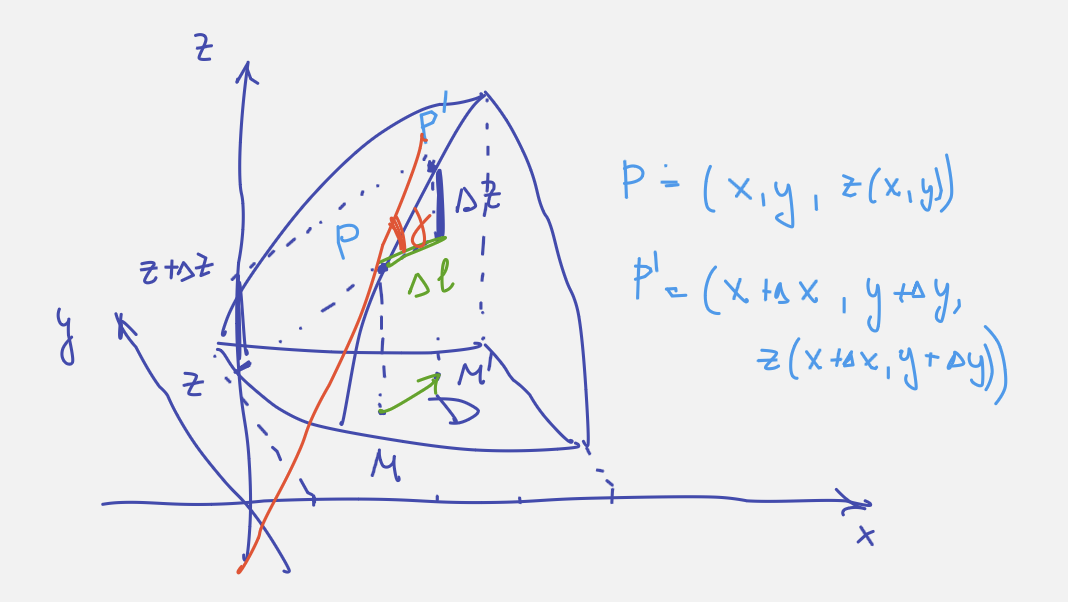
\includegraphics[width=.3\textwidth]{vecp.png}
\end{center}
Теорема (о производной функции по направлению)
\begin{equation}
    z=z(x,y),\ z,z'_x,z'_y - \text{непрерывна}\ => \ \pdv{z}{l} = \pdv{z}{x}cos\alpha+\pdv{z}{y}cos\beta, (cos\alpha;cos\beta) = \overline{l^o} = \frac{\overline{l}}{|\overline{l}|}
\end{equation}
Доказательство
\begin{equation*}
    \Delta_lz = \pdv{z}{x}\Delta x+ \pdv{z}{y}\Delta y + \alpha(\Delta l)\Delta x + \beta (\Delta l)\Delta y\ | :\Delta x
\end{equation*}
\begin{equation*}
    \frac{\Delta_lz}{\Delta l} = \pdv{z}{x}\frac{\Delta x}{\Delta l}+ \pdv{z}{y}\frac{\Delta y}{\Delta l} + \alpha(\Delta l)\frac{\Delta x}{\Delta l} + \beta (\Delta l)\frac{\Delta y}{\Delta l}\ | :\Delta l
\end{equation*}
\begin{equation*}
    \frac{\Delta_lz}{\Delta l} = \pdv{z}{x}\cdot cos\alpha+ \pdv{z}{y}\cdot cos\beta + \alpha(\Delta l)\cdot cos\alpha + \beta (\Delta l)\frac{\Delta y}{\Delta l}\ | :\Delta l
\end{equation*}
\begin{equation*}
    \Delta l -> 0\ => \ \Delta x -> 0,\ \Delta y-> 0
\end{equation*}
\begin{equation*}
    \pdv{z}{l} = \pdv{z}{x}\cdot cos(\alpha)+ \pdv{z}{y}\cdot cos\beta
\end{equation*}
\begin{equation*}
    \measuredangle \overline{l}= \overline{i}= (1;0)
\end{equation*}
\begin{equation*}
    \pdv{z}{l} = \pdv{z}{x}\cdot 1 +\pdv{z}{y}\cdot 0 = \pdv{z}{x}
\end{equation*}
\\
\begin{equation*}
    u  = u(x;y;z)\ \overline{l} = (l_x, l_y, l_z)\ \overline{l^o} = (cos\alpha; cos \beta; cos \gamma)
\end{equation*}
\begin{equation*}
    \pdv{u}{l} = \pdv{u}{x}cos\alpha + \pdv{u}{y}cos\beta + \pdv{u}{z}cos\gamma
\end{equation*}
\section{Частные производные высших порядков}
\begin{equation*}
    z = z(x;y);\ \pdv{z}{x} = z'_x(x;y);\ \pdv{z}{y} = z'_y(x;y)\ 
\end{equation*}
\begin{equation*}
    \pdv{^2z}{x^2} = \pdv{}{x}(\pdv{z}{x}) = (z_x')_x' = z_{xx}''(x;y) 
\end{equation*}
Теорема (о смешаных производных)
\begin{equation}
    z = z(x;y),\ z, z'_x, z'_y, z''_xy, z''_yx\ - \text{ непрерывны }=>\ \pdv{^2z}{x\partial y}= \pdv{^2z}{y\partial x}
\end{equation}

\section{Дифферинциалы высших порядков}
\begin{equation}
    z = z(x;y)
\end{equation}
Первого порядка
\begin{equation*}
    dz = \pdv{z}{x}dx + \pdv{z}{y} dy = \left(\pdv{}{x}dx + \pdv{}{y}dy\right)z
\end{equation*}
Второго порядка
\begin{equation*}
    d^2z = d(dz) = d\left(\pdv{z}{x}dx + \pdv{z}{y} dy\right) = \left(\pdv{^2}{x^2}dx^2 + 2\pdv{^2}{x\partial y }dxdy + \pdv{^2}{y^2}dy^2\right)z
\end{equation*}
\begin{equation*}
    d^n z = d(dz) = \left(\sum_{k=0}^{n}C_n^k\pdv{^n}{x^{n\cdot k}\partial y^k}dx^{n-k}dy^k\right)z
\end{equation*}
Функция о трёх переменных
\begin{equation}
    u = u(x;y;z)
\end{equation}
\begin{equation*}
    du = \left(\pdv{}{x}dx+\pdv{}{y}dy+\pdv{}{z}dz\right)u
\end{equation*}

\section{Экстремумы функции нескольких функций}
\begin{equation*}
    z =z(x,y);\ M_0\ \ z(x,y)\ \ \text{eкстремум, если}
\end{equation*}
\begin{equation*}
    z(x,y) \leq z(x_0, y_0) <=> \Delta z(x_0, y_0) \leq 0 \-\ max
\end{equation*}
\begin{equation*}
    z(x,y) \geq z(x_0, y_0) <=> \Delta z(x_0, y_0) \geq 0 \-\ min
\end{equation*}
$M_0 $ - точка экстремума
\\ \\
$M_0$ - Критическая для функции z, если для неё все частные производные первого порядка == 0 или не существуют
\\ \\
$M_0$ - стационарная точка для функции z, если для неё все частные производные  == 0
\\ \\ 
\textbf{Теорема(необходимое условие экстремума)}
\begin{equation*}
    M_0(x_0; y_0) - point\ extremum\ for\ z(x;y)\ => M_0-\ \text{Критическая}
\end{equation*}
Досказательство

\begin{center}
    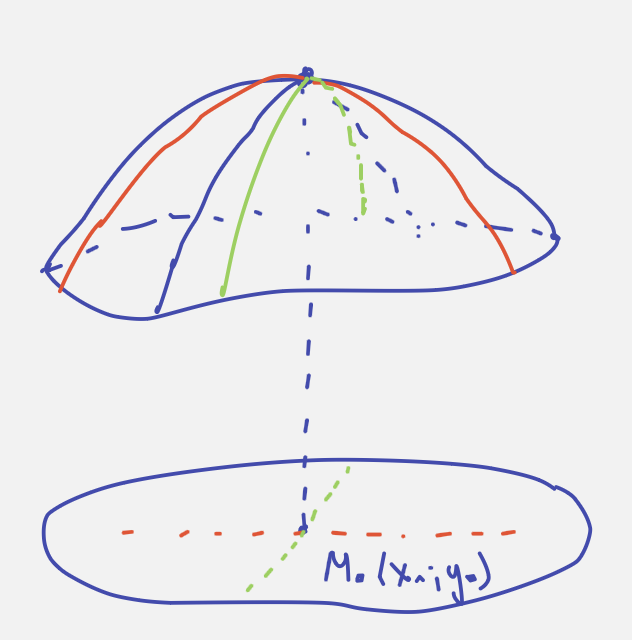
\includegraphics[width=.3\textwidth]{feixed} 
\end{center}
\begin{equation*}
    1) y = y_0\ (fixed)
\end{equation*}
\begin{equation*}
    z_0(x, y_0) = \phi (x)
\end{equation*}
\begin{equation*}
    x_0 - \ \text{ точка экстремума функции}\ \phi (x)
\end{equation*}
\begin{equation*}
    x_0 - \ \text{ критическая для }\ \phi (x): \phi'(x_0) = 0
\end{equation*}
\begin{equation*}
=> z'_x(x; y_0) = 0
\end{equation*}
\begin{equation*}
    2) x = x_0 -\ fixed
\end{equation*}
\begin{equation*}
    z = (x_0; y) = \psi (y)
\end{equation*}
\begin{equation*}
    y_0 - \text{точка критическая для } \psi(y)
\end{equation*}
\begin{equation*}
    => y_0 - \text{точка критическая для } \psi(y) : \psi'(y_0)=0\ => z'_y(x_0;y_0)=0
\end{equation*}
1+2 => $M_0(x_0;y_0)$ - точка критическая для z(x;y)
\\ \\
\textbf{Теорема(достаточные условия экстремума для стационарной точки)}
\begin{equation*}
    z(x; y)\ M_0 - ctachionarnaya
\end{equation*}
Пусть z и её частные производные до 2-го порядка включены непрерывно в окрестность $M_0$
\begin{equation*}
    z''_{xx}(M_0) = A,\ z''_{xy}(M_0) = B,\ z_{yy}''(M_0)=C
\end{equation*}
\begin{equation*}
   D=AC-B^2 = 
   \begin{cases}
    A&B\\
    B&C
   \end{cases}
\end{equation*}
\begin{equation*}
    D>0\ and \ A<0\ =>\ M_0-\ max
 \end{equation*}
 \begin{equation*}
    D>0\ and \ A>0\ =>\ M_0-\ min
 \end{equation*}
 \begin{equation*}
    D<0,\ M_0 - \text{седловая}
 \end{equation*}
 \begin{equation*}
    D=0,\ ? \text{требуются доп исследования}
 \end{equation*}
Доказательство
 \begin{equation*}
    z(x+\Delta x; y+\Delta y) = z(x;y)+ \frac{dz(x;y)}{1!}+\frac{d^2z(x;y)}{2!}+0(\Delta \rho^2)\ \ Teylor
 \end{equation*}
 \begin{equation*}
= z(x;y) + (z_x'(x;y)\Delta x+z'_y(x;y)\Delta) + \frac{1}{2!}(z''_{xx}(x;y)(\Delta x)^2+2\cdot z''_{xy}(x;y)\Delta x\Delta y+z''_{yy}(x;y)(\Delta y)^2) + o((\Delta \rho)^2)
\end{equation*}
$M_0 $ - стационарная => dz($M_0 $)=0
\begin{equation*}
    \Delta z(M_0)=\frac{1}{2!}(A(\Delta x)^2+2B\Delta x\Delta y + C(\Delta y)^2)+o((\Delta \rho)^2)
\end{equation*}
\begin{equation*}
    \Delta x = \Delta \rho \cdot cos\phi\ \ and \Delta y = \Delta \rho \cdot sin\phi\
\end{equation*}
(**)
\begin{equation*}
    = \frac{(\Delta \rho)^2}{2}(A\cdot cos^2\phi + 2B\cdot cos\phi\cdot sin \phi + C\cdot sin^2\phi + \frac{o(\Delta \rho ^2)}{\Delta \rho^2})
\end{equation*}
\begin{equation*}
    (A^2\cdot cos^2\phi + 2AB\cdot cos\phi\cdot sin \phi + B^2sin^2\phi)+(AC-B^2)sin^2\phi
\end{equation*}
(*)
\begin{equation*}
    \frac{1}{A}(((A\cdot cos\phi + B\cdot sin \phi)^2)+(AC-B^2)sin^2\phi)
\end{equation*}
\begin{equation*}
    1) (AC-B^2)=D>0\ \ A<0\ => \Delta z(M_0)\leq 0 \ \ \Delta \rho -> 0 \max
\end{equation*}
\begin{equation*}
    2) (AC-B^2)=D>0\ \ A>0\ => \Delta z(M_0)\geq 0 \ \ \Delta \rho -> 0 \min
\end{equation*}
\begin{equation*}
    3) (AC-B^2)=D<0\ 
\end{equation*}
\begin{equation*}
    3.1) (AC-B^2)=D<0\ \ A>0\ \ \phi: sin\phi = 0\ \ (*)=\frac{A^2}{A} = A \ >0\ \ => \Delta z(M_0)\geq 0
\end{equation*}
\begin{equation*}
    \phi: tg\phi = -\frac{A}{B}\ \ (*)=\frac{1}{A}(AC - B^2)\cdot sin^2\phi\ \ => \ \Delta(M_0)\leq 0 
\end{equation*}
no extremum
\begin{equation*}
    3.2) \ A<0\:
\end{equation*}
no extremum
\begin{equation*}
    3.3) A=0: (**)= sin \phi(2b\cdot cos\phi+c\cdot sin\phi);\ \phi > 0 \text{знак как B};\ \phi < 0 \text{знак как -B}
\end{equation*}
\begin{equation*}
    4) D=0:\ \Delta z(M_0)=\frac{(\Delta \rho)^2}{2}(\frac{(Acos\phi + Bsin\phi)^2}{A}+o(1))
\end{equation*}
\begin{equation*}
    \phi: tg\phi = - \frac{A}{B}\ => \Delta z (M_0) = (\Delta\rho)^2\cdot o(1) = o(\Delta\rho^2)
\end{equation*}
нужны доп исследования
\end{document}
